\chapter{Distributed Document Embeddings}
\label{chapter:distembed}
In this chapter we describe the concept of distributed word and document embeddings and why distributed representations of words and documents are better than one-hot or bag-of-words representations as described in \ref{sec:textrepr}. We then give a background on different models that learn distributed representations for words in a fully unsupervised manner and finally describe in detail our proposed model for learning distributed embeddings for documents that can be used for multi-label text classification.

\section{Motivation}
\label{sec:motivation_distributed}
\todo{Get in tune to document representations. Say words and documents suffer in the same manner with one-hot or bow representations. Express problems in docs with changing words. Give example of sentence}

\todo{Can be tackled with distributed repr. Similarity measures as simple as cos-distance can be introduced in documents. Lets model joint distributions of words with continuous distributions. Words have distributed representaions but not docs. }

Words are regarded as atomic symbols in most rule-based and statistical natural language processing(NLP) tasks and hence need the appropriate representation to solve the NLP tasks with greater ease and accuracy. 
Words are traditionally expressed as one-hot vectors, i.e. as vectors of the size of the vocabulary where exactly one element is $1$ and the rest all are zero.
Though these representations have been widely used, one-hot representations have a plethora of drawbacks that pose problems and limit the ability of systems to perform better. 
\begin{enumerate}
\item \textbf{Curse of Dimensionality} : One-hot representations lead word vectors to be the size of the vocabulary which often consists of tens to hundereds of thousands of words. Due to this curse of dimensionality, language modelling becomes almost impossible where the number of parameters would grow exponentially with the size of the vocabulary if the words are represented as one-hot vectors.

\item \textbf{No Word Similarity} : As words are represented by sparse orthogonal vectors, there is no notion of word similarity that can be introduced. In one-hot representation, the word ``symphony'' is equally close to the words ``bark'' and ``guitar''. We would want word representations such that they capture the semantic or topical similarity between words.
\end{enumerate}

Due to the problems dicussed above there is a need for more robust, low-dimensional, non-sparse vector representations for words that capture the semantic similarity between them, can be used to model language with continuous distributions and can be used as inputs for various other NLP tasks. 

\section{Background}
\label{sec:background_distributed}
Distributed word representations are dense fixed-sized feature vectors learnt for words in an unsupervised manner from large text corpus that capture the semantic similarity between words. Each word $w_{i}$ in the corpus is represented by a vector, $v_{w_{i}} \in \mathbb{R}^{m}$, where $m$ usually ranges from $50-300$. These dense representations help deal with sparsity and high-dimensionality issues in ont-hot representations and also provide provision for estimating similarities between words; which is as simple as taking the dot-product or calculating the cosine-distance between the vectors. 

All of the word vector learning models make use of neural networks  ( \citep{bengio2003neural}, \citep{mnih2013learning}, \citep{mikolov2013distributed}, \citep{collobert2011natural}, \citep{bottou2014machine}, \citep{turian2010word}, \citep{levy2014dependencybased} ) but differ in their training objectives. 

Below we describe in detail two models to show how models with very different learning objectives and architechture can lead to learning high-quality word vectors.

\subsection{Neural Probabilistic Language Model (NPLM)}
\label{sec:bengio}
Introduced by \cite{bengio2003neural}, their model aims to learn distributed word vectors and a probability function that uses these vectors to learn a statistical model of language. In their model, the probability of a word sequence is expressed as the product of conditional probabilities of the next word given the previous ones. 
\begin{equation}
P(w_{1}^{T}) =  \prod_{t=1}^{T} P(w_{t}| w_{1}^{t-1})
\end{equation}
And making the n-gram assumption, 
\begin{equation}
P(w_{t} | w_{1}^{t-1}) \approx P(w_{t} | w_{t-n+1}^{t-1})
\end{equation}
i.e. the probability of the next word in the sequence is mostly affected by the local context, in this the previous $n$-words and not the whole past sequence.

Their model maps each word to a $m$-dimensional vector in a matrix $C \in \mathbb{R}^{|V|\times m}$ and estimates the probability $P(w_{t} = i|w_{t-n+1}^{t-1})$ i.e. the probability that the $t^{th}$ word in the sequence is $w_{i}$. The neural network that is used to estimate this probability using the word vectors is shown in Figure~\ref{fig:nn:bengio}
\begin{figure}[t!]
    \centering
        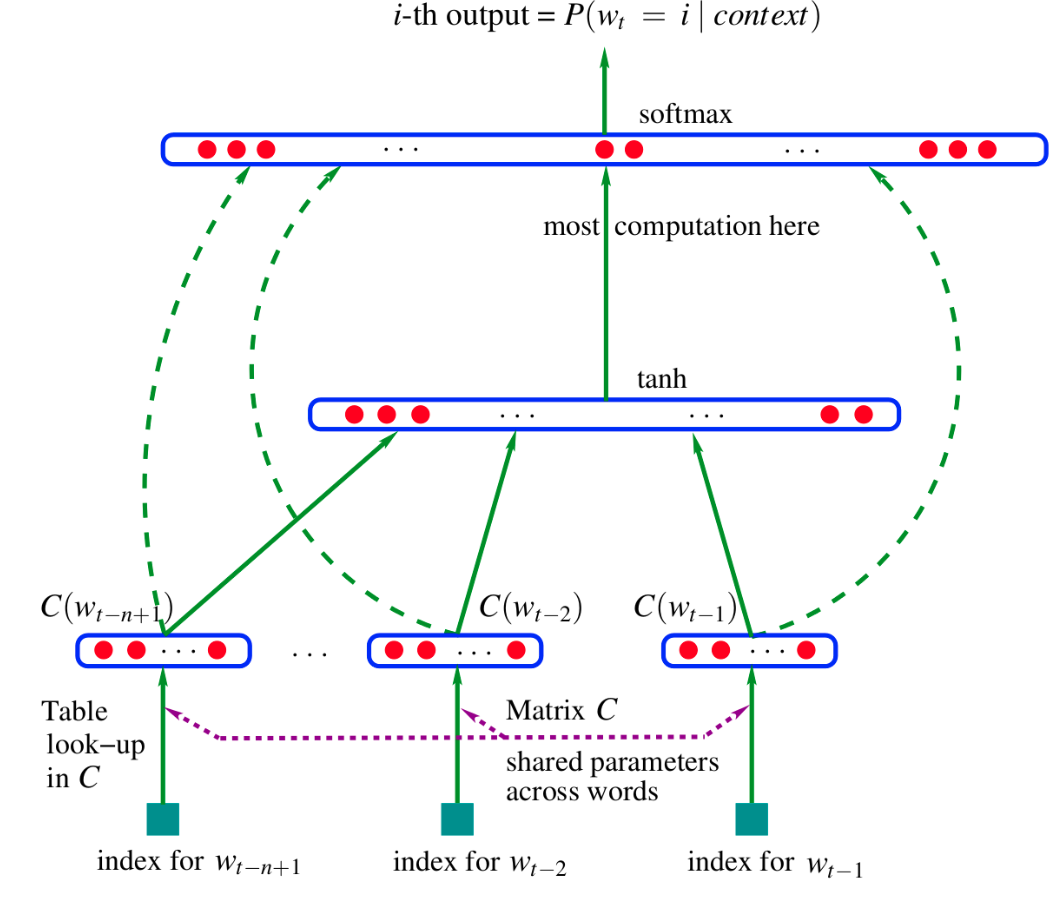
\includegraphics[width=0.8\textwidth]{figs/bengio_nn.png}
    \caption{Bengio's Neural Network Architechture for Neural Probabilistic Language Model}
    \label{fig:nn:bengio}
\end{figure}
For each input sequence, the neural network outputs a vector $y \in \mathbb{R}^{|V|}$, where $y_{i}$ is the unnormalized log-probability that the $t^{th}$ word in the sequence is $w_{i}$.
\begin{equation}
y = b + Wx + Utanh(d + Hx)
\end{equation}
where $tanh$ is the hyperbolic tangent applied to introduce non-linearity and $x$ is the word feature layer activation vector constructed by the concatenation of the context word vectors,
\begin{equation}
x = (C(w_{t-1}), C(w_{t-2}), \ldots, C(w_{t-n+1}))
\end{equation}
The unnormalized log probabilities in $y$ are converted to positive probabilities summing to $1$ by using a \emph{softmax} output layer that computes, 
\begin{equation}
P(w_{t} = i | w_{t-1}, \ldots, w_{t-n+1}) = \frac{e^{y_{w_t}}}{\sum_{i}e^{y_{i}}}
\end{equation}
The parameters of the model $(b, d, W, U, H)$ and the word vectors $C$ are estimated by maximizing the log-likelihood of the training corpus.

\subsection{Log-Linear Models : word2vec}
\label{sec:word2vec}
Simple log-linear models are proposed in \cite{mikolov2013efficient} as opposed to the non-linear NPLM model to bring down the training time complexity without sacrificing with the quality of the word vectors. The models bring down the complexity of learning vectors by not having a non-linear layer and matrix weighting of the input vectors that are the costliest operations in NPLM. The two models proposed in \cite{mikolov2013efficient} are,

\begin{itemize}
\item{\textbf{Continuous Bag-of-Words (CBOW) model}} : This model is different from the NPLM in that the projection layer is shared for all words; i.e. all words get projected into the same hidden layer vector (their vectors are averaged). This architechture hence neglects the ordering of the words as opposed to NNLM that uses the concatenation of input vectors for the projection layer. The training criteria in this model is to to classify the current (middle) word given its context. It also uses word sequence from the future to aid this task with the relaxation that the aim is not to learn a language model. The model archtitechture is given in Figure~\ref{fig:nn:cbow}.
\begin{figure}[h!]
    \centering
        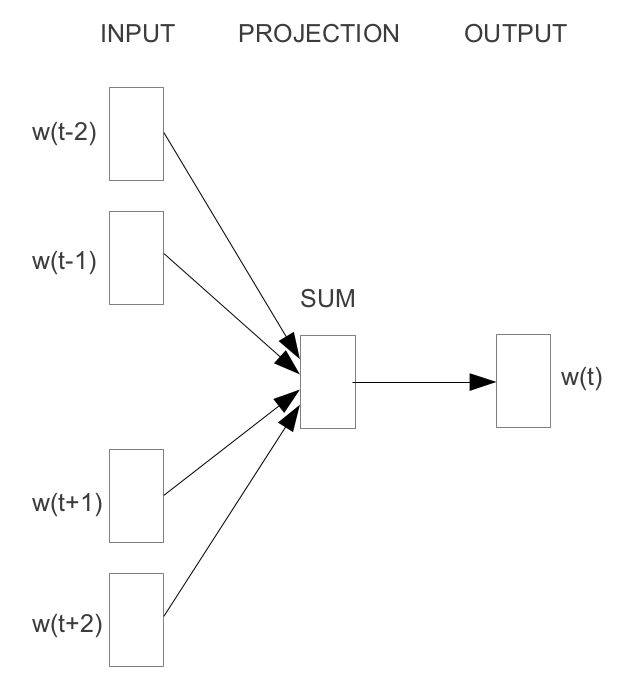
\includegraphics[width=0.5\textwidth]{figs/mikolov_cbow.png}
    \caption{Continuous Bag-of-Words Model (CBOW) \todo{Add ref?}}
    \label{fig:nn:cbow}
\end{figure}
The model first computes the hidden layer vector $h$, 
\begin{equation}
h(w_{t-k}, \ldots, w_{t+k}) = \frac{w_{t-k} + \ldots + w_{t-1} + w_{t+1} + \dots + w_{t+k}}{2k}
\end{equation}
where, $w_{t-i}$ is the $i$-th previous word in the context of the middle word $w_{t}$ and $k$ is the window length.
The neural network then computes a unnormalized log-probability vector $y$ similar to Sec.\ref{sec:bengio}, and uses the \emph{softmax}-classifier to estimate $P(w_{t}|w_{t-k}, \ldots, w_{t+k})$,
\begin{equation}
y = b + Uh(w_{t-k}, \ldots, w_{t+k})\\
\end{equation}
\begin{equation}
\label{eq:cbow:prob}
P(w_{t}|w_{t-k}, \ldots, w_{t+k}) = \frac{e^{y_{w_t}}}{\sum_{i} e^{y_{i}}}
\end{equation}
The parameters of the CBOW model, $(b, U)$ and the word vectors ($w_{i}$) are learnt by maximizing the average log probability (Eq.~\ref{eq:cbow:prob}) of the training corpus.

\item{\textbf{Continuous Skip-gram model}} : This model is similar to the CBOW model, but instead of predicting the middle word based on the context, it tries to maximize the classification of a word based on another word in the context. More precisely, given each word, the skip-gram model tries to predict words within a certain range before and after the current word. The model architechture is given in Figure~\ref{fig:nn:skip}
\begin{figure}[h!]
    \centering
        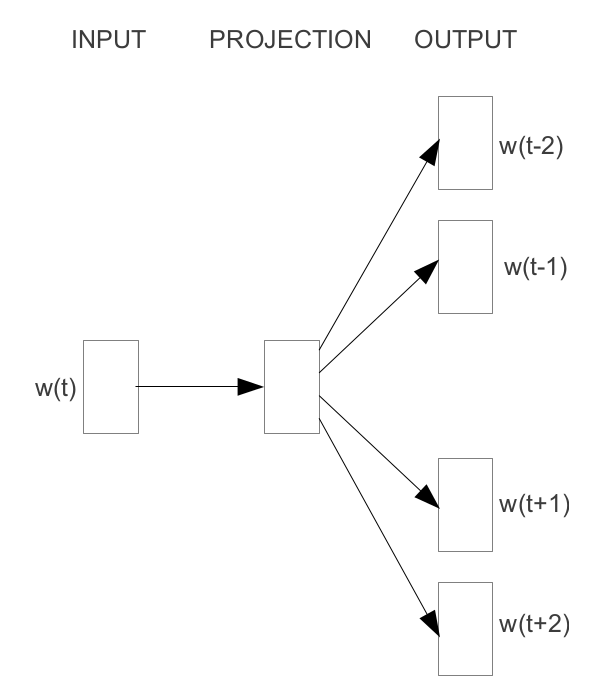
\includegraphics[width=0.4\textwidth]{figs/mikolov_skip.png}
    \caption{Continuous Skip-gram Model \todo{Add ref?}}
    \label{fig:nn:skip}
\end{figure}
Formally, given a sequence of words in a context $w_{t-k}, \ldots, w_{t+k}$, the skip-gram model defines $P(w_{t+j}|w_{t})$ using the \emph{softmax}-classifier in the following manner,
\begin{equation}
\label{eq:skip:prob}
P(w_{t+j}|w_{t}) = \frac{\exp{(v_{w_{t}} \cdot v_{w_{t+j}} )} }{\sum_{i} \exp{(v_{w_{t}} \cdot v_{w_{i}})} }
\end{equation}
The only parameters of the Skip-gram model are the word vectors ($v_{w_{i}}$) that are learnt by maximizing the average log probability (Eq.~\ref{eq:skip:prob}) of predicting all the context words for all the words in the training corpus.
\end{itemize}
The CBOW and the Skip-gram models use the \emph{hierarchical softmax} \citep{morin2005hierarchical} instead of the full softmax to speed-up the learning process.

\section{Distributed Document Embeddings : Our Approach}
\label{sec:ourapproach}


